
\section{Supplementary material}


\subsection{Descriptive statistics}

\small
\renewcommand{\arraystretch}{1.3}
\begin{longtable}{p{7cm} p{1cm} p{0.8cm} p{0.8cm} p{0.8cm} p{0.8cm} p{0.8cm} p{0.8cm} p{0.8cm} p{0.8cm}}
\caption{Descriptive statistics for all patients arriving at each stroke team. The table shows summary statistics across all stroke teams.}\\
\toprule
\endhead
Statistic & Stroke teams & mean & Std Dev & min & 25\% & 50\% & 75\% & max\tabularnewline
\midrule
Yearly admissions & 119 & 509 & 208 & 95 & 372 & 489 & 627 & 1183\tabularnewline
Age (mean) & 119 & 74 & 2 & 65 & 73 & 75 & 76 & 78\tabularnewline
Proportion aged 80+ & 119 & 0.40 & 0.06 & 0.20 & 0.36 & 0.40 & 0.44 & 0.51\tabularnewline
Proportion male & 119 & 0.53 & 0.02 & 0.47 & 0.51 & 0.53 & 0.55 & 0.60\tabularnewline
Prior disability (mRS, mean) & 119 & 1.02 & 0.25 & 0.29 & 0.87 & 1.03 & 1.21 & 1.60\tabularnewline
Proportion prior disability (mRS) 0-2 & 119 & 0.81 & 0.05 & 0.67 & 0.78 & 0.81 & 0.84 & 0.97\tabularnewline
Proportion ischaemic stroke & 119 & 0.88 & 0.02 & 0.83 & 0.86 & 0.88 & 0.89 & 0.93\tabularnewline
Stroke severity (NIHSS, mean) & 119 & 7.0 & 1.0 & 4.6 & 6.3 & 7.2 & 7.8 & 9.1\tabularnewline
Proportion with known onset & 119 & 0.68 & 0.14 & 0.43 & 0.58 & 0.67 & 0.76 & 1.00\tabularnewline
Onset-to-arrival time (minutes, median) & 119 & 204 & 76 & 109 & 155 & 180 & 224 & 466\tabularnewline
Proportion arriving within 4 hours known onset & 119 & 0.38 & 0.06 & 0.19 & 0.34 & 0.38 & 0.43 & 0.51\tabularnewline
Proportion with precisely known onset & 119 & 0.33 & 0.11 & 0.01 & 0.28 & 0.34 & 0.39 & 0.63\tabularnewline
Proportion onset during sleep & 119 & 0.14 & 0.06 & 0.00 & 0.09 & 0.14 & 0.17 & 0.34\tabularnewline
Proportion arrive by ambulance & 119 & 0.78 & 0.07 & 0.47 & 0.76 & 0.79 & 0.82 & 0.92\tabularnewline
Call-to-ambulance arrival time (minutes, median) & 113 & 22 & 10 & 13 & 17 & 20 & 24 & 103\tabularnewline
Ambulance on scene time (median) & 113 & 31 & 3 & 20 & 28 & 31 & 33 & 41\tabularnewline
Ambulance conveyance time (minutes, median) & 113 & 18 & 5 & 10 & 15 & 17 & 21 & 37\tabularnewline
Arrival-to-scan time (minutes, median) & 119 & 53 & 21 & 13 & 39 & 51 & 63 & 129\tabularnewline
Proportion receiving thrombolysis & 119 & 0.115 & 0.034 & 0.021 & 0.092 & 0.110 & 0.136 & 0.245\tabularnewline
Scan-to-thrombolysis time (minutes, median) & 119 & 34 & 10 & 14 & 28 & 34 & 41 & 72\tabularnewline
Discharge disability (mRS, mean) & 119 & 2.641 & 0.352 & 1.361 & 2.413 & 2.699 & 2.900 & 3.320\tabularnewline
Proportion discharged mRS 0-2 & 119 & 0.524 & 0.095 & 0.293 & 0.454 & 0.522 & 0.594 & 0.799\tabularnewline
Proportion discharged mRS 5-6 & 119 & 0.195 & 0.037 & 0.095 & 0.170 & 0.198 & 0.218 & 0.287\tabularnewline
\bottomrule
\label{tab:hospital_stats_1}
\end{longtable}
\normalsize

\small
\begin{longtable}{p{7cm} p{1cm} p{0.8cm} p{0.8cm} p{0.8cm} p{0.8cm} p{0.8cm} p{0.8cm} p{0.8cm} p{0.8cm}}
\caption{Descriptive statistics for patients arriving at each stroke team, for patients arriving within 4 hours of known stroke onset. The table shows summary statistics across all stroke teams.}\\
\toprule
\endhead
Statistic & Stroke teams & mean & Std Dev & min & 25\% & 50\% & 75\% & max\tabularnewline
\midrule
Yearly admissions & 119 & 193 & 78 & 28 & 139 & 183 & 241 & 428\tabularnewline
Age (mean) & 119 & 75 & 2 & 66 & 73 & 75 & 76 & 79\tabularnewline
Proportion aged 80+ & 119 & 0.41 & 0.06 & 0.23 & 0.37 & 0.41 & 0.45 & 0.57\tabularnewline
Proportion male & 119 & 0.53 & 0.03 & 0.45 & 0.51 & 0.53 & 0.55 & 0.64\tabularnewline
Prior disability (mRS, mean) & 119 & 1.04 & 0.25 & 0.37 & 0.88 & 1.04 & 1.22 & 1.60\tabularnewline
Proportion prior disability (mRS) 0-2 & 119 & 0.80 & 0.06 & 0.66 & 0.77 & 0.81 & 0.83 & 0.95\tabularnewline
Proportion ischaemic stroke & 119 & 0.85 & 0.03 & 0.75 & 0.84 & 0.85 & 0.87 & 0.94\tabularnewline
Stroke severity (NIHSS, mean) & 119 & 8.9 & 1.1 & 6.4 & 8.2 & 9.0 & 9.7 & 11.4\tabularnewline
Proportion with known onset & 119 & 1.00 & 0.00 & 1.00 & 1.00 & 1.00 & 1.00 & 1.00\tabularnewline
Onset-to-arrival time (minutes, median) & 119 & 105 & 9 & 85 & 100 & 105 & 111 & 132\tabularnewline
Proportion arriving within 4 hours known onset & 119 & 1.00 & 0.00 & 1.00 & 1.00 & 1.00 & 1.00 & 1.00\tabularnewline
Proportion with precisely known onset & 119 & 0.62 & 0.17 & 0.02 & 0.54 & 0.66 & 0.75 & 0.91\tabularnewline
Proportion onset during sleep & 119 & 0.05 & 0.05 & 0.00 & 0.01 & 0.03 & 0.06 & 0.30\tabularnewline
Proportion arrive by ambulance & 119 & 0.89 & 0.07 & 0.54 & 0.87 & 0.91 & 0.93 & 0.98\tabularnewline
Call-to-ambulance arrival time (minutes, median) & 110 & 19 & 5 & 8 & 16 & 18 & 21 & 51\tabularnewline
Ambulance on scene time (median) & 110 & 28 & 4 & 20 & 26 & 28 & 31 & 46\tabularnewline
Ambulance conveyance time (minutes, median) & 110 & 17 & 4 & 9 & 14 & 16 & 20 & 28\tabularnewline
Arrival-to-scan time (minutes, median) & 119 & 27 & 11 & 4 & 21 & 28 & 34 & 100\tabularnewline
Proportion receiving thrombolysis & 119 & 0.293 & 0.070 & 0.111 & 0.250 & 0.282 & 0.333 & 0.534\tabularnewline
Scan-to-thrombolysis time (minutes, median) & 119 & 34 & 10 & 14 & 28 & 34 & 40 & 71\tabularnewline
Discharge disability (mRS, mean) & 119 & 2.803 & 0.353 & 1.507 & 2.609 & 2.837 & 3.039 & 3.663\tabularnewline
Proportion discharged mRS 0-2 & 119 & 0.494 & 0.094 & 0.209 & 0.424 & 0.495 & 0.554 & 0.771\tabularnewline
Proportion discharged mRS 5-6 & 119 & 0.236 & 0.045 & 0.138 & 0.208 & 0.231 & 0.256 & 0.420\tabularnewline
\bottomrule
\label{tab:hospital_stats_2}
\end{longtable}
\normalsize

\small
\begin{longtable}{p{7cm} p{1cm} p{0.8cm} p{0.8cm} p{0.8cm} p{0.8cm} p{0.8cm} p{0.8cm} p{0.8cm} p{0.8cm}}
\caption{Descriptive statistics for patients arriving at each stroke team, for patients arriving by ambulance within 4 hours of known stroke onset. The table shows summary statistics across all stroke teams.}\\
\toprule
\endhead
Statistic & Stroke teams & mean & Std Dev & min & 25\% & 50\% & 75\% & max\tabularnewline
\midrule
Yearly admissions & 119 & 173 & 74 & 15 & 125 & 163 & 227 & 400\tabularnewline
Age (mean) & 119 & 75 & 2 & 66 & 74 & 76 & 77 & 81\tabularnewline
Proportion aged 80+ & 119 & 0.43 & 0.06 & 0.24 & 0.39 & 0.43 & 0.47 & 0.62\tabularnewline
Proportion male & 119 & 0.52 & 0.03 & 0.45 & 0.51 & 0.52 & 0.54 & 0.60\tabularnewline
Prior disability (mRS, mean) & 119 & 1.10 & 0.25 & 0.46 & 0.94 & 1.09 & 1.26 & 1.66\tabularnewline
Proportion prior disability (mRS) 0-2 & 119 & 0.79 & 0.06 & 0.65 & 0.75 & 0.79 & 0.83 & 0.93\tabularnewline
Proportion ischaemic stroke & 119 & 0.85 & 0.03 & 0.75 & 0.83 & 0.85 & 0.87 & 0.94\tabularnewline
Stroke severity (NIHSS, mean) & 119 & 9.4 & 1.2 & 6.7 & 8.6 & 9.5 & 10.2 & 12.2\tabularnewline
Proportion with known onset & 119 & 1.00 & 0.00 & 1.00 & 1.00 & 1.00 & 1.00 & 1.00\tabularnewline
Onset-to-arrival time (minutes, median) & 119 & 106 & 10 & 84 & 99 & 105 & 112 & 151\tabularnewline
Proportion arriving within 4 hours known onset & 119 & 1.00 & 0.00 & 1.00 & 1.00 & 1.00 & 1.00 & 1.00\tabularnewline
Proportion with precisely known onset & 119 & 0.62 & 0.17 & 0.02 & 0.54 & 0.65 & 0.75 & 0.92\tabularnewline
Proportion onset during sleep & 119 & 0.05 & 0.05 & 0.00 & 0.01 & 0.03 & 0.06 & 0.33\tabularnewline
Proportion arrive by ambulance & 119 & 1.00 & 0.00 & 1.00 & 1.00 & 1.00 & 1.00 & 1.00\tabularnewline
Call-to-ambulance arrival time (minutes, median) & 110 & 19 & 5 & 8 & 16 & 18 & 21 & 51\tabularnewline
Ambulance on scene time (median) & 110 & 28 & 4 & 20 & 26 & 28 & 31 & 46\tabularnewline
Ambulance conveyance time (minutes, median) & 110 & 17 & 4 & 9 & 14 & 16 & 20 & 28\tabularnewline
Arrival-to-scan time (minutes, median) & 119 & 26 & 11 & 4 & 20 & 25 & 33 & 95\tabularnewline
Proportion receiving thrombolysis & 119 & 0.300 & 0.072 & 0.130 & 0.252 & 0.289 & 0.345 & 0.537\tabularnewline
Scan-to-thrombolysis time (minutes, median) & 119 & 34 & 10 & 13 & 27 & 33 & 40 & 73\tabularnewline
Discharge disability (mRS, mean) & 119 & 2.926 & 0.352 & 1.867 & 2.717 & 2.928 & 3.150 & 3.819\tabularnewline
Proportion discharged mRS 0-2 & 119 & 0.465 & 0.096 & 0.184 & 0.398 & 0.462 & 0.524 & 0.696\tabularnewline
Proportion discharged mRS 5-6 & 119 & 0.254 & 0.051 & 0.147 & 0.221 & 0.253 & 0.280 & 0.486\tabularnewline
\bottomrule
\label{tab:hospital_stats_3}
\end{longtable}
\normalsize



\subsection{Model confusion matrices}

\subsubsection{Thrombolysis choice model}


\begin{figure}
    \centering
    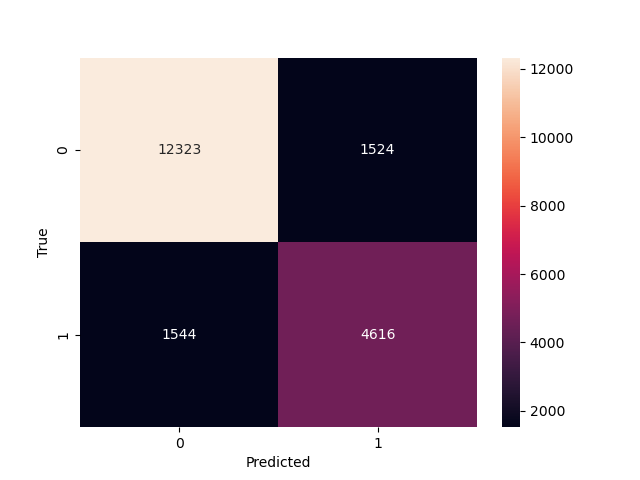
\includegraphics[width=0.75\linewidth]{images/confusion_matrix_choice}
    \caption{Enter Caption}
    \label{fig:confusion_choice}
\end{figure}

\begin{figure}
    \centering
    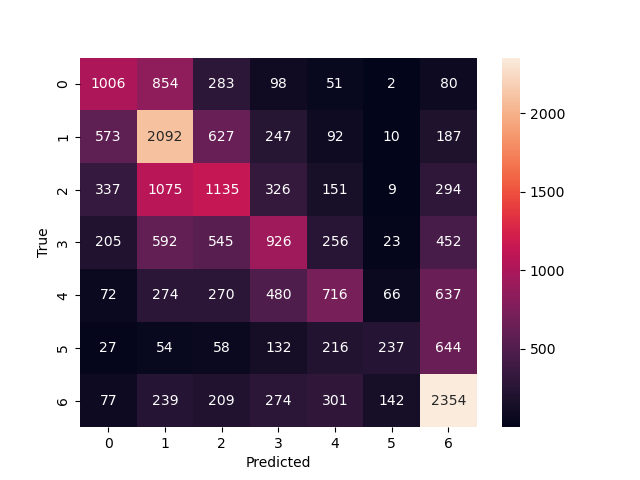
\includegraphics[width=0.75\linewidth]{images/confusion_matrix_outcome}
    \caption{Enter Caption}
    \label{fig:confusion_outcome}
\end{figure}


